\documentclass[authoryear]{elsarticle}
\usepackage{latexsym}
%\usepackage{rotate}
\usepackage{graphics}
\usepackage{amsmath}
\usepackage{amssymb}
\usepackage{comment}
\bibliographystyle{chicago}



\newcommand{\logit}{\mathrm{logit}}
\newcommand{\I}{\mathrm{I}}
\newcommand{\E}{\mathrm{E}}
\newcommand{\p}{\mathrm{P}}
\newcommand{\e}{\mathrm{e}}
\newcommand{\vecm}{\mathrm{vec}}
\newcommand{\kp}{\otimes}
\newcommand{\diag}{\mathrm{diag}}
\newcommand{\cov}{\mathrm{cov}}
\newcommand{\eps}{\epsilon}
\newcommand{\ep}{\varepsilon}
\newcommand{\obdots}{\ddots}    % change this later
\newcommand{\Ex}{{\cal E}}
\newcommand{\rat}{{\frac{c_{ij}}{c_{i,j-1}}}}
\newcommand{\rmu}{m}
\newcommand{\rsig}{\nu}
\newcommand{\fd}{\mu}
\newcommand{\tr}{\mathrm{tr}}
\newcommand{\cor}{\mathrm{cor}}
\newcommand{\bx}[1]{\ensuremath{\overline{#1}|}}
\newcommand{\an}[1]{\ensuremath{a_{\bx{#1}}}}

\newcommand{\bi}{\begin{itemize}}
\newcommand{\ei}{\end{itemize}}

\renewcommand{\i}{\item}
\newcommand{\sr}{\ensuremath{\mathrm{SRISK}}}
\newcommand{\cs}{\ensuremath{\mathrm{CS}}}
\newcommand{\cri}{\ensuremath{\mathrm{Crisis}}}
\newcommand{\var}{\ensuremath{\mathrm{VaR}}}
\newcommand{\covar}{\ensuremath{\mathrm{CoVaR}}}
\newcommand{\med}{\ensuremath{\mathrm{m}}}
\newcommand{\de}{\mathrm{d}}
\renewcommand{\v}{\ensuremath{\mathrm{v}_q}}
\newcommand{\m}{\ensuremath{\mathrm{m}}}
\newcommand{\tvar}{\ensuremath{\mathrm{TVaR}}}



\newcommand{\eref}[1]{(\ref{#1})}
\newcommand{\fref}[1]{Figure \ref{#1}}
\newcommand{\sref}[1]{\S\ref{#1}}
\newcommand{\tref}[1]{Table \ref{#1}}
\newcommand{\aref}[1]{Appendix \ref{#1}}




\newcommand{\cq}{\ , \qquad}
\renewcommand{\P}{\mathrm{P}}
\newcommand{\Q}{\mathrm{Q}}

\newcommand{\Vx}{{\cal V}}
\newcommand{\be}[1]{\begin{equation}\label{#1}}
\newcommand{\ee}{\end{equation}}




\begin{document}

% Title of paper
\title{Systemic risk and contagion effects in Australian financial institutions and sectors}
% List of authors, with corresponding author marked by asterisk
\author{Piet de Jong,  Geoff Loudon and Weihao Choo \\[4pt]
% Author addresses
\textit{Department of Applied Finance and Actuarial Studies\\ Macquarie University, Sydney, NSW 2109.}
\\[2pt]
%E-mail address for correspondence
{piet.dejong@mq.edu.au}}

% Running headers of paper:
\markboth%
% First field is the short list of authors
{De Jong}
% Second field is the short title of the paper
{Systemic risk}

\maketitle

\section{Literature review}

The starting point for the proposed research is the recent literature and the CIFR targeted areas and APRA aims and functions.
This recent literature includes the following
\cite{adrian2011covar},
\cite{acharya2012capital},
\cite{acharya2012measuring}
and \cite{brownlees2010volatility}.   The proposed research aims to extend and apply these techniques particularly in relation to the entities regulated by APRA.   Thus our  broad aim is to develop, implement and bring to bear recent developments in stress testing  on the aims of APRA and the CIFR targeted research areas detailed above.   

\section{Improved  measures of contagion and systematic risk}
\renewcommand{\c}{\ensuremath{\mathrm{CoVaR_q}}}
\renewcommand{\v}{\ensuremath{\mathrm{VaR}_q}}

$\covar_q$ as proposed in \cite{adrian2011covar} is a basis for proposed measures contagion, exposure and systemic risk.   It  suffers from a number of drawbacks:
\bi
\i Couched in terms of $\var_q$ containing the scale of the original measurements.   It is worthwhile to have measures and techniques robust to scale.
\i  Conditioning  on $\var_{0.5}$ is undesirable and relatively intractable.  In our proposal we reference stress with respect  to the unconditional $\var_q$.   This permits a more transparent analysis and estimation. 
\i  Our proposed approach  separates out scale effects and interdependence effects and aims to  relates these separately to external variables including shocks and drivers of systemic risk.   Thus $\var_q$ movements due to scale are disentangled from movements due to codependence with separate driver responses.
\ei

\section{Significance of the project and  policy implications}

Understanding the impact of external shocks and their propagation through   the financial system is vital for managing and remediating systemic risk. Effective regulation is dependent upon the development of a robust and reliable set of appropriate risk measures.  We propose new measures of systemic risk that relate marginal and joint distributions separately to external drivers. This allows for more cogent and coherent stress testing as it includes the estimation of contagion effects, exposure effects and systemic risk across related entities and different financial sectors. Improved stress testing, estimation of risk effects and transmission of shocks through the financial system will make for more cogent prudential policy, prudential margin setting and better identify sources of risk to the financial system.

\newcommand{\q}{\mathrm{Q}}
\section{Percentile sensitivity and contagion}\label{perc}

\subsection{Theorem}  Suppose $x$ is a random vector with marginal distributions\footnote{To economise on notation, write $F_j(x)\equiv F_j(x_j)\equiv F(x_j)$ and similar for other vector functions.} 
$$
F(x)\equiv \{F(x_1),\ldots ,F(x_p)\} \equiv (u_1,\ldots,u_p)\equiv u\ .
$$ 
Further suppose $0\le q\le 1$ is given and  $\q(x)$ is the vector of $q$--quantiles
$$
F\{\q(x)\}=q1=\q(u)\ ,
$$
where $1$ is a vector of $p$ ones. 
Define the stress vector with respect to $x_j$ as\footnote{In \cite{adrian2011covar}  $\Delta CoVar_q\equiv q_{y|x=q_x}-q_y$.  Variable $y$  is generally the ``financial system" and hence considered is the change in the \v\ of the system when institution $x$ stressed, with stress  interpreted as $x=q_x$.  On page 10 of their paper they incorrectly state ``... $CoVaR$ conditions on the event that [an] institution is at its VaR level, which occurs with probability $q$."} 
\be{stress}
\frac{\de\q(x)}{\de x_j} \equiv \q(x|u_j>q) - \q(x)\ ,
\ee
where $\q(x|u_j>q)$ is the vector of $q$--quantiles of $x$ given $u_j>q$.    Then if $\q(x)$  is linear in $q$ 
 then
\be{implicit}
\frac{\de\q(x_i)}{\de\q(x_j)} \equiv \frac{\de\q(x_i)/\de x_j}{\de\q(x_j)/\de x_j} =  
\frac{f_j}{f_i} 
 \frac{q_{ij}}{q(1-q)}\cq q_{ij}=C_{ij}(q+q_{ij},q) - q^2\ ,
\ee
where $f_i$ and $f_j$ are the densities of $x_i$ and $x_j$ evaluated at $\q(x_i)$ and $\q(x_j)$ and  $C_{ij}$ is the copula of $(u_i,u_j)$.   
Further if 
$$
s_{ij}\equiv \frac{q_{ij}}{q(1-q)}\ ,
$$ then  $-1\le s_{ij}\le 1$ with $s_{ij}=\pm 1$ if $x_i$ and $x_j$ are comonotonic and counter monotonic, respectively.  If $x_i$ and $x_j$ are independent then  $s_{ij}=0$. If $u_i$ and $u_j$ are exchangeable  then  $s_{ji}=s_{ij}$.

\subsection{Proof}

By definition
$$
\frac{\de\q(u_i)}{\de u_j} \equiv \q(u_i|u_j>q) -q \equiv q_{ij}\ ,
$$
where  $q_{ij}$ is such that
\be{Qdef}
q =  \frac{\P(u_i\le  q+q_{ij},u_j>q)}{1-q}  = \frac{ q+q_{ij}-C_{ij}(q+q_{ij},q)}{1-q}\ ,
\ee
Rearranging yields the second equation in \eref{implicit}.
Now
 \be{first}
 \frac{\de\q(x_i)}{\de x_j}\equiv \q_{q+q_{ij}}(x_i) - \q(x_i) \approx \q'(x_i)q_{ij}= \frac{q_{ij}}{f_i} \ ,
 \ee
where $'$ denotes differentiation with respect to $q$ and the subscript on $\q$ indicates the revised $q$ for the quantile calculation.  The approximation follows from a first order Taylor expansion and is exact if the quantile is linear in $q$.   Similarly
 \be{second}
 \frac{\de\q(x_j)}{\de x_j}\equiv  \q_{q+q(1-q)}(x_j) - \q(x_j)\approx \frac{q(1-q)}{f_j}\ .
 \ee
 Dividing \eref{first} by \eref{second} yields the first equation in  \eref{implicit} and completes the proof.

\subsection{Discussion}  The critical  result is that sensitivities factor into contributions from the ratios of the marginal densities and quantities calculated from the pairwise copulas.  The via  the implicit  equation for $q_{ij}$ in \eref{implicit}, solved using a  root finding algorithm.
  The quantities $q_{ij}$ are implicitly defined from the pairwise copulas. In summary the ``sensitivity" matrix 
$$
S \equiv \frac{\de Q(x)}{\de Q'(x)}\ ,
$$
where $'$ denotes transposition has ones on the diagonal quantities between $\pm 1$ off the diagonal.   The matrix $S$ is called the sensitivity matrix and displays the sensitivity of the $q$--quantile of  each component of $x$ to  stress in the same or other components.  

Since $f_i$ and $f_j$ are  the densities evaluated at $\q(x_i)$ and $\q(x_j)$  it follows that the ratio $f_i/f_j$ can be replaced by the ratio of the hazards.   This is  useful in cases were it is practical to model the hazard rather than the density.


\subsection{Implementation}

\fref{fig1} displays the empirical copulas calculated from four weekly closing stock prices labelled anz, cba, mcq and  wbc for $n=761$ weeks from 2000 April 12 through to 2014 October 29.  The empirical copulas are calculated by converting each observation to an empirical percentile and plotting the same against each of the other series percentiles.  

\begin{figure}
  \begin{center}
    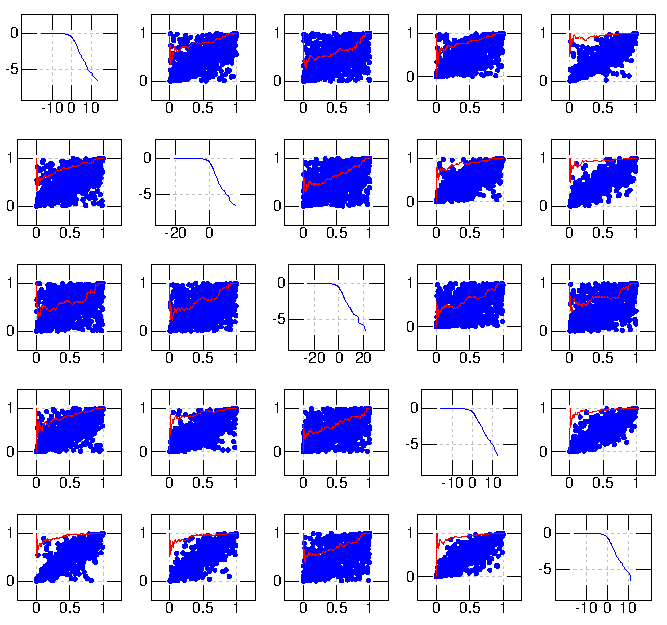
\includegraphics{fig1.pdf}
    \caption{Pairwise copulas of bank stocks  cba, anz, mqg, wbc, and the overall bank index.  Red lines plot sensitivity $s_{ij}$ as a function of $q$.}\label{fig1}
   \end{center}
\end{figure}


To estimate  $q_{ij}$  at a particular $q$, the second equation in \eref{implicit} is iterated\footnote{The second equation in \eref{implicit} is a contraction mapping and hence has a fixed point.} starting from $q_{ij}=0$ where copulas are estimated as 
$$
\hat C_{ij}(u_i,u_j) \equiv \hat\E\{(p_{ik}\le u_i)(p_{jk}\le u_j)\}\ .
$$
Here $\hat\E$ computes the empirical mean over the cases $k=1,\ldots,n$ and $p_{ik}$ and $p_{jk}$ are the empirical percentiles  of case $k$ of $x_i$ and $x_j$, respectively.

\subsection{Generalisations}
\renewcommand{\r}{\mathrm{R}}
Similar results apply when $\Q(x)$ is replaced by  other risk measures such as $\r(x)\equiv\E\{xr(u)\}$ where $r$ is a given function which acts componentwise and $xr(u)$ denotes componentwise multiplication.  For example if $r(u)=mu^{m-1}$ then  $\r(x)=\E\{\max(x^1,\ldots,x^m)\}$ where  $x^1,\ldots,x^m$ are $m$ independent copies of $x$ and the risk measure is the expected worst outcome in $m$ independent trials.

With $\r(x)$, the analogue of \eref{stress} is 
\be{stress2}
\frac{\de\r(x)}{\de x_j} \equiv \r(x|u_j>r_j) - \r(x_j)\cq r_j\equiv\p\{x_j\le\r(x_j)\} \ .
\ee
This differs from \eref{stress}  in that a different risk measure is used and  $r_j$ replaces $q$.   If  the components of $\r(x)$ are linear in the $r_i$ then
\be{implicit2}
\frac{\de\r(x_i)}{\de\r(x_j)} =  
\frac{f_j}{f_i} 
 \frac{q_{ij}}{q(1-q)}\cq q_{ij}=C_{ij}(r_i+q_{ij},r_j) - r_ir_j\ ,
\ee
where $f_i$ and $f_j$ are the $x_i$ and $x_j$ densities at the $r_i$ and $r_i$ quantiles, respectively. 

\section{Partially Gaussian copulas}

Suppose $(u,v)=F_*(x,y)$  where $x$ and $y$ are scalar random variables.    Suppose $0<u_1<\cdots<u_n<1$  are   ordered observed values of $u$ and $q_t=\Phi^-(u_t)$, $t=1,\ldots,n$.  The correspondingly ordered values of $v$ and $z=\Phi^-(v)$ are denoted $v_t$ and $z_t$.  Note $\Ex(z_t)=\Ex(q_t)=0$ and $\Ex(z^2_t)=\Ex(q^2_t)=1$ where $\Ex$  is the empirical mean. 

Smoothing methods are here proposed to smooth and simulate $y$ values  using a copula on $(u,v)$ constructed via    a cubic spline model linking $z$ and $u$.   Of particular concern are simulated $z$ when $u$ is  near $0$ or $1$ corresponding to  $x$ extremes.    Given a simulated $u$ and in turn $z$, $(x,y)=F^-_*\{u,\Phi(z)\}$, a draw from the joint.  Constraining $u$ draws to say the upper tail, yields corresponding upper tail values for $y$.   The challenge is to produce cogent $z$'s or $y$'s that properly reflect dependence in different parts of the distribution unencumbered by inappropriate constraints, and in particular tail constraints, inherent in say the Gaussian copula setup.    Practical methods admit fitting on the basis of observed data, and testing procedures for  departures or otherwise from Gaussianity.   The method outlined below achieves this.

\begin{comment}
   The simulation singles out independent and dependent variables.   Which should be which?  If $x$ and $y$ are actual time series the simulation $(x_t,\hat y_t)$ is ordered back into the original time series order.
\end{comment}

The partially Gaussian  (PG) copula for $(u,v)$ is stated in terms of  $q\equiv\Phi^-(u)$ and $z\equiv\Phi^-(v)$ on the grid   $u_t=t/(n+1)$, $t=1,\ldots,n$ with 
\be{cusp}
z_t = \alpha_t+\beta q_t+ sh_t\eps_t\cq \alpha_{t+1}=\alpha_t +\delta_t+1.268\eta_t\cq \delta_{t+1}=\delta_t+\eta_t\ .
\ee
Here $\eps_t$ and $\eta_t$ are serially and contemporaneously uncorrelated zero mean disturbances with common variance $\sigma^2$.  The  $q_t$ term is the   Gaussian component and  $\alpha_t$ a nonparametric deviation.   

The parameter $s$ controls overall smoothness while  $h_t\ge 0$,  controlling the variability at different $t$ determines local smoothness.
In particular if $s=0$ then the signal $\alpha_t+\beta q_t$ is forced to reproduce every  $z_t$ while $h_t=0$ implies reproduction at the particular $t$.     If $h_t$ is large then little notice is taken of $z_t$ and the fitted signal at $t$ is relatively smooth.  Thus $s$ controls overall smoothness of the signal and  $h_t$ the smoothness at a particular $t$.  Comparability between models and fits is facilitated by normalising $h_t>0$ such that the average  is 1.  


The Gaussian copula is where $\alpha_t$ and $h_t$ are  identically 0 and  1, respectively, implying  $(z_t,q_t)$ with $t$ uniform on $1,\ldots,n$  is bivariate normal  with correlation $\beta=\pm\sqrt{1-(s\sigma)^2}\equiv\rho$.    

Thus $\alpha_t$ provides for a nonparametric extension of the Gaussian copula.   The nature of the extension is spelt out in the  second and third equations in \eref{cusp} where $\alpha_0$ and $\delta_0$ are assumed unknown.  If $\sigma\rightarrow 0$, equivalent to $s\rightarrow\infty$,  the first equation in \eref{cusp} is
$
z_t = \alpha_0+\delta_0 t + \beta q_t + s\eps_t
$.
With this linear formulation for $\alpha_t$,  $\beta=\rho$ if $\alpha_0=\delta_0=0$.    Model \eref{cusp} with  $\beta=0$ is the  nonparametric model since $z_t$ is varies smoothly with $t$, unrelated to $q_t$.  If $\beta=0$ and $\sigma\rightarrow 0$ there is a probit relationship between $z_t$ and $u_t$.  Finally $s=0$ implies $\alpha_t+\beta q_t=z_t$ for any $\beta$.   The full range of possibilities is set out in \tref{pg} discussed in more detail below.  The function $\alpha_t$ is thought of as an intercept function. 

The $\alpha_t=0$ and $\alpha_t=\alpha_0+\delta_0 t$ specifications are generalised by supposing $\alpha_t$ is twice differentiable and minimising
\be{spline}
 \sum_{t=1}^n\left(\frac{z_t-\alpha_t-\beta q_t}{h_t}\right)^2 + s^2\int_{-\infty}^{\infty} \left(\alpha_t''\right)^2\de t\ .
\ee
with respect to $\alpha_t$ and $\beta$.
 In \eref{spline} the $h_t$  weighs fitting errors: a large  $h_t$ at a particular $t$ implies  error at $t$ is largely ignored while small $h_t$ implies  error at $t$ is  minimized at all cost.  The function $a_t$ and scalar $b$ minimising \eref{spline} deliver a function $a_t+bq_t$ where $a_t$ is piecewise twice differentiable and $a_t+bq_t$ passes closest to, in a mean square error sense, to $z_t$  with a penalty $s^2$ for  roughness measured in terms of the second derivative.   At the minimum, the first term in \eref{spline} is $(s\sigma)^2$.   \cite{Brown&DeJong:2001} demonstrate the equivalence of \eref{cusp} and \eref{spline}.

The  function $\alpha_t$ minimising \eref{spline}  is, at integer $t$,  $a_t=\E(\alpha_t|z_1,\ldots,z_n)$  computed with \eref{cusp} where $\eps_t$ and $\eta_t$ are normal, 0 mean, variance $\sigma^2$ random variables and $q_t$ fixed.  Between integer $t$,  the  minimum is quadratic in $t$.  A useful feature is that $\beta$ is simultaneously estimated alongside $a_t$ as the generalised least squares estimate under \eref{cusp}.  All calculations under \eref{cusp} provide error covariance matrices as detailed and applied below.  

\section{Special cases of the PG model}  

Special cases of  \eref{cusp}  are displayed in \tref{pg}.   In \eref{cusp}, if $s\rightarrow\infty$ then $\sigma\rightarrow 0$   since the variance of $z_t$ is finite.    Thus $s\rightarrow\infty$  implies the noise to signal ratio becomes large where noise refers to   $s\eps_t$ and signal to $\eta_t$, the error term driving  the smooth component $\alpha_t$.   As the noise to signal ratio $s$ increases, less of the variation in $z_t$ is explained by $\alpha_t$.  In the limit $\sigma$ is zero implying $\alpha_t=\alpha_0+\delta_0 t$, as straight line.   The further restriction $\alpha_0=\delta_0=0$ forces $\alpha_t$ identically zero.



The first row in \tref{pg} is the  Gaussian copula.  In this setup $\alpha_t$ is identically zero: there is no  signal component.  The additional restriction $\beta=0$ eliminates the Gaussian component $q_t$.  Co (or counter) monotonicity results in the Gaussian framework if $\rho=\pm 1$ as displayed in the third row.
If $s= 0$ then there is no measurement noise and the combined signal $\alpha_t+\beta q_t$ must pass through the points $z_t$ resulting in a perfect fit.   In terms of \eref{spline}, $s=0$ implies there is no roughness penalty and hence the minimisation is solely focussed on minimising the first, squared error, term, achieved  by setting $\alpha_t+\beta q_t=z_t$. 
 
 \begin{table}[htdp]
\caption{Special cases of the PG copula; in all cases $\rho\equiv\pm\sqrt{1-(s\sigma)^2}$}\label{pg}
\begin{center}
\begin{tabular}{l|c|ccccc|l}
\hline
case& $\alpha_t$ & $\beta$ &$s$ & $\sigma$ & $\alpha_0$&$\delta_0$  & other\\
\hline
Gaussian & 0 &  & $\infty$ & $0$&  0&0 &$\rho=\beta$\\
independence &  0 & 0 & $\infty$&0 & 0 &0 &$\rho=0$\\
$\pm$comonotonic  & 0 &$\pm 1$ &0 & 0 &0 & 0 &$z_t=\pm q_t$  \\
empirical  & $z_t$ &  & $0$  &  &   &  &$\rho=1$ \\ 
linear probit &$\alpha_0(1-2u_t)$&  0 &  $\infty$ &0& & $\frac{-2\alpha_0}{n+1}$ &indep. if $\alpha_0=0$\\
nonparametric & $\E(z_t|u_t)$  & 0 & & & &  & non Gaussian \\
PG & $\E(z_t-\beta q_t|u_t)$ & & & & & &  \\
\hline
\end{tabular}
\end{center}
\end{table}%

The linear probit row in \tref{pg}  eliminates the Gaussian component $q_t$ by setting $\beta=0$, and giving maximum penalty for rougness.   The resulting prediction  is a straight line $\hat z_t=\alpha_0+\delta_0 t$.  However the mean of the $z_t$ and hence $\hat z_t$ is zero implying $0=\alpha_0 + \delta_0(n+1)/2$.   Solving for $\delta_0$ gives the $\delta_0$ constraint displayed in \tref{pg} and the resulting straight line signal $\alpha_t$.

The bottom row of \tref{pg} displays the general partial Gaussian specification absent  any constraints on the parameters.  Eliminating the Gaussian component from the signal by setting $\beta=0$ leads to the nonparametric, non Gaussian specification in the second last row of \tref{pg}.

\section{Overall and global correlation}

\cite{bjerve1993correlation} state ``The local regression slope, which focuses on change in expected $y$ as $x$ changes, may be of greater interest than expected  $y$ for a given $x$." They go on to argue for  a  ``scale--free standardised version of the local regression slope."\footnote{The scale free feature conflicts with the calculations below where  slope differs according to whether it is with respect to $t$ compared to $q_t$.  Hence the noise terms must also be affected by the transformation in a way not apparent in the expressions below.} Their suggested measure  in  the current notation is 
\be{rhot}
 \rho_t\equiv\pm\left\{1+\left(\frac{\psi_t}{s\sigma h_t}\right)^{-2}\right\}^{-\frac{1}{2}}\ ,
\ee
where $s$, $\sigma$ and $h_t$ are as in \eref{cusp} or \eref{spline} and $\psi_t$ is the regression slope at $t$ as set out below.  The ratio $\psi_t/(s\sigma h_t)$ is a signal to noise ratio and a high value implies $\rho_t\approx \pm 1$.    In general the signal  $\psi_t$ is the local slope of the relationship while $s\sigma h_t$ is a measure of local noise.   The sign of $\rho_t$ is discussed in the context of particular choices of signal $\psi_t$.  

With the Gaussian copula 
$$
z_t=\beta q_t + (\sqrt{1-\rho^2})\varepsilon_t\ ,
$$
where $\varepsilon_t$ is standard normal.  In this  case the nonparametric component $\alpha_t$ is excluded.  The slope with respect to $q_t$ is constant $\psi_t=\beta=\rho$ and the noise variance $s\sigma h_t=\sqrt{1-\rho^2}$ constant across $t$ and \eref{rhot} reduces to $\rho_t=\rho$ for all $t$.  The Gaussian copula case is displayed in the first row of the of \tref{corr}.

\begin{table}[htdp]
\caption{Overall and local correlations.  In all cases $\hat\rho=\sqrt{1-\Ex\{(z_t-\hat z_t)^2\}}$}\label{corr}
\begin{center}
\begin{tabular}{l|ccc|l}
\hline
case & $\psi_t$ & $q_t$ & $\alpha_t$ & estimates\\
\hline\hline
Gaussian & & & \\
-- overall,  local &$\rho=\beta$ &$\checkmark$& $\times$ & $\hat\rho=\Ex(z_tq_t)$ \\
\hline
nonparametric & & & \\
-- overall &$\rho$ &$\times$ & $\checkmark$& $\hat\rho$ from $\widehat{\mathrm{PG}}(\beta=0)$\\
-- local  &$n\phi(q_t)\delta_t$ &$\times$ & $\checkmark$& $\hat\delta_t$ from $\widehat{\mathrm{PG}}(\beta=0)$\\
\hline
PG & & & \\
-- overall & $\rho$ & $\checkmark$& $\checkmark$& $\hat\rho$ from $\widehat{\mathrm{PG}}$ \\
-- local & $n\phi(q_t)\delta_t+\beta$&$\checkmark$& $\checkmark$&$\hat\beta$, $\hat\delta_t$ from $\widehat{\mathrm{PG}}$  \\
\hline\hline
\end{tabular}
\end{center}
\end{table}%

The second set of row in \tref{corr} is the nonparametric Gaussian copula where, in \eref{cusp},  $\beta=0$.  Hence $q_t$ is removed and  the relationship between $z_t$ and $t$ or $u_t$ is  modelled in terms of the  nonparametric component $\alpha_t$.  The   slope $\alpha_{t+1}-\alpha_t$  at  $t$ is, apart from error,
$\delta_t$.   However $\delta_t$ is the slope with respect to $t$ and required is the slope with respect to $q_t$:
\be{normslope}
\psi_t=\frac{\de \alpha_t}{\de q_t} = \left( \frac{\de u}{\de t}\frac{\de q_t}{\de u}\right)^{-1}\frac{\de \alpha_t}{\de t}  \approx
\left\{\frac{1}{n\phi(q_t)}\right\}^{-1}\delta_t  = n\delta_t\phi(q_t)\ ,
\ee
where $\phi$ is the standard normal density.    

The final set of rows in \tref{corr} deals with the general PG case.   As in the other situations, the overall correlation $\rho$ is derived from the overall fit.   The overall correlation exceeds that derived from both the specialised Gaussian and nonparametric cases.   The higher overall correlation is partialed out locally according to both nonparametric and parametric components.   In any PG fit $\hat\beta$ will differ from the Gaussian copula estimate $\Ex(z_tq_t)$.  

If $s=0$ then $s\eps_t=0$  and  the signal to noise ratio is infinite implying $\rho_t=1$ for all $t$.  Thus the empirical and comonotonic cases imply, as expected,  $\rho_t=\pm 1$.   With the linear probit model $\sigma=0$ and $\alpha_t=\alpha_0(1-2u_t)$ with slope with respect to $u_t$ of $-2\alpha_0$ and
\be{normslope2}
\psi_t =  \left( \frac{\de q_t}{\de u_t}\right)^{-1}\frac{\de \alpha_t}{\de u_t}  =
 -2\alpha_0\phi(q_t)\cq  \rho_t\equiv\pm\left[1+\left\{\frac{2\alpha_0\phi(q_t)}{s\sigma h_t}\right\}^{-2}\right]^{-\frac{1}{2}}\ ,
\ee
If $h_t$ is constant then  local correlation is  highest if  $q_t=0$ and monotonically declines towards zero as $q_t$ moves away from zero. 

The above $\psi_t$ and implied correlations are for the $(q,z)$ scale.  However the local correlations also apply on the $(u,v)$ scale since the transformation from $u$ to $q$ and $v$ to $z$ are the same inverse normal probability transform and slopes are identical\footnote{This also follows since local correlation is independent of scale.}
$$
\frac{\de v}{\de u} =\left(\frac{\de z}{\de v}\right)^{-1} \frac{\de z}{\de q} \frac{\de q}{\de u} = \frac{\de z}{\de q}\ .
$$ 
\section{Simulating from the PG copula} 

To explain simulation with the PG model, consider initially  simulating from a special case: the Gaussian model.   Given data $(q_t,z_t)$, $t=1,\ldots,n$ where
$q_t=\Phi(u_t)$ and $u_t=t/(n+1)$ suppose 
\be{rhohat}
\tilde z_i\sim N(\hat\rho \tilde q_i,1-\hat\rho^2)\cq \hat\rho=\Ex(z_tq_t) = \E(\rho|  z)\cq \tilde q_i\sim N(0,1)\ ,
\ee
where $z\equiv(z_1,\ldots,z_n)$,  remaining fixed in the subsequent discussion.
Simulating $\tilde q_i$ multiple times produces multiple $\tilde z_i$ while $\hat\rho$  remains fixed.   To ensure  coverage, the $\tilde q_i$ are chosen successively as $q_1,\ldots,q_n$.   The  $n$ pairs $(u_i, \tilde v_i)$ where $\tilde v_i=\Phi(\tilde z_i)$, $i=1,\ldots,n$  are $n$ independent draws with   uniform  empirical distribution for the $u_i$ and approximately uniform empirical distribution for the $\tilde v_i$.   Repeatedly cycling over $i=1,\ldots,n$  produces an unlimited supply of  draws.

The PG generalisation of the Gaussian copula simulation  is repeatedly cycling over  $i=1,\ldots,n$ with 
\be{rhohat2}
\tilde z_i\sim N(a_i+bq_i, s^2\sigma^2)\ , \ \ \ \  a_i=\E(\alpha_i|  z)\ , \ \ \ \ b=\E(\beta|  z)\ .
\ee
The $a_i$ and $b$ and estimate of $\sigma$ are calculated with the Kalman Filter Smoother (KFS)  \citep{DeJong:91a} while $s$ is set to achieve desired smoothness.  Alternatively $s$ is estimated as discussed in \sref{xx}.  In  \eref{rho2} the $a_i$, $q_i$  and $b$ remain fixed across cycles, analogous to fixing $\hat \rho$  in the  Gaussian copula simulation.   

Iterations \eref{rhohat} and \eref{rhohat2}  ignore  estimation variability in $\hat\rho$ or $a_i$ and $b$.  This shortcoming is addressed by varying  $a_i$ and $b$  across  each cycle 
$$
\tilde a_i \sim N\{\E(\alpha_i|  z),\cov(\alpha_i|  z)\}\cq  \tilde b\sim N\{\E(\beta|  z),\cov(b|  z)\}\ ,
$$
and using these  in the first relation of \eref{rhohat2}  instead of $a_i$ and $b$.
The conditional expectations and covariance matrices are recursively calculated with the KFS while consistant  draws  across $i$  are made with the 
simulation smoother extension  \citep{DeJong&Shephard:95}. 

\section{Factor PG copula model}

The PG  model is stated in terms of the generic variable $q_t=\Phi^-(u_t)$ where $u_t=t/(n+1)$, $t=1,\ldots,n$.   The sole relevance of $x_t=F_x^-\{\Phi(q_t)\}$   on  $y_t=F^-_y\{\Phi(z_t)\}$ is on  the ordering  of $y_t$: once  $y_t$  is ordered using $x_t$, the latter has no further import.  This suggest a vector extension  to the PG model.

Suppose $y_t$ is a $p$--vector with components $y_{it}$, $i=1,\ldots,p$ with $y_t$ is observed for $t=1,\ldots n$.   Suppose each component series in $y_t$ is ordered according to $x_t$, a scalar series observed or inferred along with the $y_{it}$.   Without loss of generality assume $y_t$, $t=1,\ldots,n$ denotes the component series after ordering with respect to $x_t$ and define $v_t$ and $z_t$ from the componentwise ordered $y_t$ as, for $t=1,\ldots,n$, 
$$
z_t = \Phi^-_*(v_t)\cq v_t = F_*(y_t)\cq q_t=\Phi^-(u_t)\cq u_t=\frac{1}{n+1}\ .
$$
In terms of this notation the one factor PG model is
\be{factor}
z_t = 1\alpha_t + \beta q_t + s\grave h_t\eps_t\cq \eps_{t} \sim N(0,\sigma^2I)\ ,
\ee
where $\alpha_t$ is  as in \eref{cusp}, $\grave h_t$ the diagonal matrix formed from vector $h_t$, and $1$,  $h_t$ and $\eps_t$ are $p$--vectors with component one,  $h_{it}$,  and $\eps_{it}$, respectively.  Further $\beta$ is vector while $s$ and $\sigma$ are scalar.

The one--factor PG model explains components of $z_t$ in terms of a common nonparametric component $\alpha_t$, a parametric Gaussian component $q_t$, and error.  Replacing $1\alpha_t$ in \eref{cusp} by a vector  $\alpha_t$ and making $s\sigma$ component specific  yields the PG model.  Variants include forcing  a common response to $q_t$ by requiring  $\beta$ to be scalar. 

The one--factor PG model is estimated in the same way as the PG model, using vector $z_t$.   In practice $x_t$, the scalar variable serving to order the components of $y_t$, is either an external driver or a composition from $y_t$.
 

\section{Below here is review/junk}

\subsection{\cite{bjerve1993correlation} review}
\begin{enumerate}
\item  Points out $\cov(z|t=t^*)\ne 0$  while $\cov\{\E(z)|t=t^*\}=0$.  So cannot form a correlation from the variation at $t$ compared to the variation in the mean -- there is no variation in the latter.
\item  Conditioning $t$ on a neighbourhood of $t^*$ and calculating the correlation in neighbourhood will lead to low correlation even if relationship is strong.  Not sure I understand this.
\item  Distinguishes between $\cov\{\E(z|t)\}/\cov(z)$ as a measure of correlation and ordinary correlation.  The former he calls Pearson correlation while Gallton--Pearson is the usual correlation.
\item  States that to the first order  both correlations are such that
$$
\cor\{z,t|t\in N_h(t^*)\}=\frac{h\beta_{t^*}}{\sqrt 3\sigma_{t^*}}
$$
where $\beta_t$ is the local regression and $\sigma_t$ the local residual? variation.
\item Then considered is
$$
\xi_{t^*} = \lim_{h \rightarrow 0}\frac{\cor\{z,t|t\in N(t^*)\}}{h/\sqrt 3} = \frac{\beta_{t^*}}{\sigma_{t^*}}
$$
that is the local slope devided by the local standard deviation.  Note I  assume the overall correlation is 1 and so $\sigma_1$ does not appear in the numerator.
\item  Maps $\xi_{t^*}$ into the unit interval
$$
\rho_{t^*}= \pm\left(1+\xi^{-2}_{t^*}\right)^{-\frac{1}{2}}= \pm\left(1+\frac{\sigma^2_{t^*}}{\beta^2_{t^*}}\right)^{-\frac{1}{2}}\ ,
$$

\end{enumerate}



Constructing local correlations requires a clear idea of what is being correlated with what.   Make sure it is with $q_t$ rather than $t$ or $u_t$.  For example 


 \tref{corr} provides local and global correlations for  the PG model.  The local correlation is

where the correlation is stated on the $u$ scale and $\tau_t$ depends on the ``explanatory" variable in the correlation.  The ratio $s\sigma h_t/\tau_t$ is a noise--to--signal ratio and \eref{rhot} converts the ratio  into a scale free regression coefficient \citep{bjerve1993correlation}, equivalent to a correlation. 

  sign is that of $\beta$ and $\tau_t$ is displayed in \tref{corr}.   If $\tau_t=\rho$ then $\rho_t=\rho$.  Note that 
the ratio $\tau_t/\sqrt{1-\rho^2}$ is a signal to noise ratio.  Further, $\tau_t\rightarrow\infty$ implies $\rho_t\rightarrow 1$ while $\tau_t\rightarrow 0$ implies $\rho_t\rightarrow 0$.

The general PG case, displayed in the first row of \tref{core}, the overall correlation or standardised regression slope reduces to $\rho$, estimated as indicated in the final column of the table.




The Gaussian model is the PG model with $\alpha_t\equiv 0$ enforced by letting $s\rightarrow\infty$ and setting $\alpha_0=\delta_0=0$.   In this case the correlation between $z_t$ and $q_t$ is $\rho_g=\beta=\pm\sqrt{1-(s\sigma)^2}$.    Note 
$$
\Ex(z_t)=\Ex(q_t)=0\cq \Ex(z_t^2)=\Ex(q_t^2)=1\ ,
$$
where $\Ex$ denotes averaging over $t$ and 
\be{ess}
 \hat\rho_g =\Ex(z_tq_t) =\pm\sqrt{1-\Ex\{(z_t-\tilde z_t)^2\}}\cq \tilde z_t\equiv\hat\rho_gq_t\ .
\ee

For the general PG model  $\rho^2\equiv 1-(s\sigma)^2$.   The correlation in this case  is estimated as 
$$
\hat\rho = \sqrt{1- \Ex\{(z_t-\hat z_t)^2\}}\ge \hat\rho_g
$$
where  $\hat z_t$ are predictions  with the PG model as outlined below.   A test for PG is  computing  the percentage drop in  average squared error when moving from the Gaussian model to the PG model: 
$$
1-\frac{\Ex\{(z_t-\hat z_t)^2\}}{\Ex\{(z_t-\tilde z_t)^2\}} = \frac{\hat \rho^2-\hat \rho^2_g}{1-\hat\rho^2_g}\ .
$$
This drop tests whether the nonparametric component $\alpha_t$ adds  explanatory power over and beyond the Gaussian component.

Testing whether the  Gaussian component adds explanatory power over and above the nonparametric component is achieved with a test of  $\beta=0$.   The parameter $\beta$ is estimated using the techniques described below but is essentially a generalised least squares estimate with a standard error provided by the calculations.    



  Conversely if $\alpha_t\equiv 0$ then all correlation is due to the Gaussian component and $\rho=\rho_g$.  In the general PG case, both components are present and $\beta$ can exceed 1 in modulus. 
The partial correlation between $z_t$ and $q_t$ after allowing for $\alpha_t$ is
\be{rhoq}
\rho_q\equiv\frac{\cov(z_t-\alpha_t,q_t,)}{\sqrt{\cov(z_t-\alpha_t)\cov(q_t)}} = \frac{\beta}{\sqrt{\beta^2+(s\sigma)^2}}=\pm\left(1+\frac{1-\rho^2}{\beta^2}\right)^{-1/2}\ ,
\ee
where the sign is that of $\beta$.  Here $q_t$ is treated as random even though in \eref{cusp} it is a fixed forcing function.  If $s\sigma\rightarrow 0$ then $\rho_q\rightarrow 1$ while $\beta=0$ implies $\rho_q=0$   
and $\alpha_t=0$  implies  $\rho_q=\rho$.  In all cases $\rho_q\ge \rho_g$ where $\rho_g$ is the correlation between $z_t$ and $q_t$ assuming $\alpha_t\equiv 0$.  

Conversely the partial correlation between $z_t$ and $\alpha_t$ after allowing for $q_t$ is The  correlation between $z_t$ and $\alpha_t$ after allowing for $q_t$ is
\be{rho2}
\rho_a\equiv\frac{\cov(z_t-\beta q_t,\alpha_t)}{\sqrt{\cov(z_t-\beta q_t)\cov(\alpha_t)}} = \left\{1+\frac{(s\sigma)^2}{\cov(\alpha_t)}\right\}^{-1/2}\ .
\ee
This is BS -- has to be done properly --.  The  overall correlation between $z_t$ and $\alpha_t$ of
$$
\frac{\cov(z_t,\alpha_t)}{\sqrt{\cov(z_t)\cov(\alpha_t)}} = \frac{\cov(z_t-\beta q_t,\alpha_t)}{\sqrt{1-\beta^2-(s\sigma)^2}} =\sqrt{1-\beta^2-(s\sigma)^2}
$$
while the nonparametric correlation is the correlation between the nonparametric component $\alpha_t$ and  $z_t$ after removing the the effect of the Gaussian component:

\begin{table}[htdp]
\caption{Correlations in PG model}\label{default}
\begin{center}
\begin{tabular}{c|ccc}
&&\\
Gaussian& $\alpha_t\equiv 0$& $\rho=\pm\sqrt{1-\beta^2}$\\
nonparametric & $\beta=0$\\
\end{tabular}
\end{center}
\end{table}%
 

   If $\beta\ne 0$ then the correlation $\rho$ is due to both the the Gaussian and nonparametric components,  $q_t$ and $\alpha_t$.

With the PG model  Gaussianity is tested by setting $s$ arbitrarily large and comparing to the situation where $s$ is optimised.

Given $\alpha_t$ and $\beta$, the local  correlation at $t$ is such that
\be{rhot2}
\rho_t^2=1-\frac{\Ex\{(z_t-\alpha_t-\beta q_t)^2\}}{\Ex\{(z_t-\rho q_t)^2\}} \approx 1-\frac{(s\sigma)^2}{\Ex\{(z_t-\rho q_t)^2\}}
\ee
Here $\Ex$ averages over $t$ values in the neighbourhood of $t$.  The numerator average squared error measures the local deviation after fitting the PG model.  The denominator average squared error measures the local deviation after fitting the Gaussian model.   Since the Gaussian model is nested within the PG model the numerator is expected to be less than the denominator and $0\le\rho_t^2\le1$.   The PG model improves on the Gaussian copula if $\rho_t^2$ is near 1.

Gaussianity is indicated if $s\sigma/\sqrt{1-\rho^2}\approx 1$ i and areas where the Gaussian inadequacy are indicated by $(z_t-\rho q_t)/(s\sigma)$.  If averaging is across all $t$ then
$$
\Ex\left(\frac{z_t-\rho q_t}{s\sigma}\right) = 0\cq \Ex\left\{\left(\frac{z_t-\rho q_t}{s\sigma}\right)^2\right\} = \frac{1-\rho^2}{(s\sigma)^2}
$$
The standardised Gauss residual is then
$$
\frac{z_t-\rho q_t}{\sqrt{1-\rho^2}}
$$




   The extend of goodness of fit depends 


This measures the contribution of the Gaussian component $q_t$ to the explanation of $z_t$ after allowing for the nonparametric component $\alpha_t$.    The local nonparametric correlation is similarly defined as the contribution of the nonparametric component $\alpha_t$ after allowing for the Gaussian component $q_t$.
$$
\rho_t^2=1-\frac{\Ex\{(y_t-\alpha_t-\beta q_t)^2\}}{\Ex\{(y_t-\beta q_t)^2\}} =  1-\frac{\Ex\{(s\eps_t)^2\}}{\Ex\{(\alpha_t+s\eps_t)^2\}} = \left\{1+\left(\frac{s\sigma}{\beta q_t}\right)^2\right\}^{-1}
$$

Given $\alpha_t$ and $\beta$, the local  correlation at $t$ is such that
$$
\rho_t^2=1-\frac{\Ex\{(z_t-\alpha_t-\beta q_t)^2\}}{\Ex\{(z_t-\alpha_t)^2\}} =  1-\frac{\Ex\{(s\eps_t)^2\}}{\Ex\{(\beta q_t+s\eps_t)^2\}} = \left\{1+\left(\frac{s\sigma}{\beta q_t}\right)^2\right\}^{-1}
$$
This measures the contribution of the Gaussian component $q_t$ to the explanation of $z_t$ after allowing for the nonparametric component $\alpha_t$.    The local nonparametric correlation is similarly defined as the contribution of the nonparametric component $\alpha_t$ after allowing for the Gaussian component $q_t$.
$$
\rho_t^2=1-\frac{\Ex\{(y_t-\alpha_t-\beta q_t)^2\}}{\Ex\{(y_t-\beta q_t)^2\}} =  1-\frac{\Ex\{(s\eps_t)^2\}}{\Ex\{(\alpha_t+s\eps_t)^2\}} = \left\{1+\left(\frac{s\sigma}{\beta q_t}\right)^2\right\}^{-1}
$$


\section{Fitting PG copulas}
 The PG is readily  fit to percentile data, and provides a practical platform for copula simulation.  This is discussed, implemented, and used in subsequent sections.  The  parameters defining a PG copula are $s$, $\beta$,  $\sigma$ and starting conditions $\alpha_0$ and $\delta_0$.  Given $s$, the other parameters have  closed form expressions calculated with the Kalman filter.  A best estimate of $s$ is derived by iterating over $s$ so as to minimise  an appropriate objective function such as least squares. 

\section{Uniform on $t$ discussion}

With \eref{cusp} the squared correlation between $z_t$ and the signal $\alpha_t+\beta q_t$ is, since the variance of $z_t$ is 1:
 $$
 \rho^2=1-(s\sigma)^2 = 1- \Ex\{(z_t-\hat z_t)^2\}\cq \hat z_t\equiv\alpha_t+\beta q_t\ .
 $$
 where $\Ex$ denotes averaging over $t=1,\ldots,n$.  Since $\Ex(z_t)=\Ex(q_t)=0$ and $\Ex(z_t^2)=\Ex(q_t^2)=1$ implying
 $\Ex(\alpha_t)=0$.  Further
 $$
 1=\Vx(z_t) = \Vx(\alpha_t+\beta q_t + s\eps_t) = \beta^2 + \Vx(\alpha_t+s\eps_t) + 2\beta\Vx(q_t,\alpha_t+s\eps_t)\ .
 $$
 
 \section{Correlational properties of the PG copula}
 
 Equation \eref{rhoq} is equivalent to  
$
\O(\rho_q) =\beta/(s\sigma)
$
where $\O(x) \equiv \pm\sqrt{x^2/(1-x^2)}$.
 
 The column headed $\rho_q$ in \tref{pg} is the partial correlation between $z_t$ and $\alpha_t$ after removing the effect of the Gaussian component $q_t$.  If $\beta=0$, there is no Gaussian component and $\rho_q=\rho$.
 
 This section considers alternative correlations.   If $s\rightarrow\infty$ and $\alpha_0=\delta_0=0$ then $\alpha_t=0$ and $\eref{cusp}$ reduces to $z_t=\beta q_t+s\eps_t$ where $s\eps_t$ has mean zero and variance $0\le (s\sigma)^2\le 1$ and $\rho=\pm\sqrt{1-(s\sigma)^2}=\beta$ is the correlation, called the overall correlation.  The overall correlation is used when using a Gaussian copula.
As many authors have pointed out Gaussian copula modelling can be misleading especially when considering correlations in the tails.
Use of model \eref{cusp} permits a more nuanced view of correlation without completely abandoning the Gaussian setup.

\subsection{Partial correlation after allowing for semiparametric component}
 

\subsection{Local correlation}

Write  $\mu_t$ and  $\sigma_t$ as the mean and standard deviation of $z_t$ for $r>t$.   Then $\mu_0=0$ and $\sigma_0=1$.   The correlation between $z_r$ and $q_r$ for $r>t$ is
$$
\rho_t= \varrho_t \frac{\mu_t-a_t}{\sigma_t}= \varrho_t \frac{1-a_t/\mu_t}{\sigma_t/\mu_t}\ ,
$$
where $a_t$ is the intercept of the least squares relation and  $\varrho_t$ is the  known coefficient of variation of $q_r$ given $r>t$.   The intercept is 0 for all $t$ if $z_t=\pm q_t$ since in this case  $\rho_t=\pm 1$, $\varrho_t=\pm \sigma_t/\mu_t$.  If $z_t$ and $q_t$ are uncorrelated then 



  As $a_t$ varies, so does $\rho_t$ with $\rho_t=0$ if $\mu_t=a_t$ and $\rho_t=\pm 1$ if  
$$
\mu_t= a_t \pm \frac{\sigma_t}{\varrho_t} \ .
$$

With the Gaussian copula $a_t=\beta q_t$

Consider the correlation between $z_t$ and $q_t$ given $q_t>q$.   This is
$$
\cov(z_t,q_t|q_t>q) = \beta\cov(q_t|q_t>q)\cq \cov(q_t|q_t>q)
$$


To compute local correlation, write $\Delta z_t\equiv z_{t+1}-z_t$ and similarly for other quantities.    Assume $t$ is given and note that 
$$
\Delta z_t =\delta_t +c\eta_t + s(\eps_{t+1}-\eps_t)+\beta\Delta q_t  \cq \Delta q_t\approx \frac{q'_t}{n+1} = \frac{\sqrt{2\pi}\e^{q_t^2/2}}{n+1}
$$
Hence
$$
\E(\Delta z_t) \approx \E(\delta_t) + \sqrt{2\pi}\e^{q_t^2/2}\E(u_t) 
$$
  Then $q_t$ is a random variable and 
$$
\cov(\Delta z_t,\Delta q_t|t) = \beta^2\cov(\Delta q_t|t)\approx (\beta q'_t)^2\cov(u_t)= \frac{(\beta\sigma)^2\pi\e^{q_t^2}}{6} 
$$$$
\cov(\Delta z_t|t) = (1+c^2 + 2s^2)\sigma^2 + \beta^2\cov(\Delta q_t|t) 
$$
This final expression assumes $\cov(\delta_t)=(n+1)\sigma^2/2$:  a random $t$ is chosen to observe the random walk. 
Hence the local correlation is 
$$
\frac{\cov(\Delta z_t,\Delta q_t)}{\sqrt{\cov(\Delta z_t)\cov(\Delta q_t)}} = \left\{1+\frac{A}{\beta^2\cov(\Delta q_t)}\right\}^{-1/2}
$$ 

The local correlation between $z_t$ and $q_t$ is 
$$
\rho_t\equiv\cor(\Delta z_t,\Delta q_t|t) =  \frac{\beta\cov(\Delta q_t)}{\sqrt{\cov(\Delta z_t|t)\cov(\Delta q_t)}}=\pm\left\{\frac{\cov(\Delta z_t|t)}{\beta^2\cov(\Delta q_t)}\right\}^{-1/2} 
$$
where ``$|t$" indicates conditioning on information up to and including time $t$.   A calculation shows writing $c=4-\sqrt 3$,
$$
\cov(\Delta z_t|t)  = (2s^2+c)\sigma^2+\beta^2\cov(\Delta q_t)\cq \cov(\Delta q_t) \approx (q'_t)^2\cov(u_t)= \frac{\sigma^2\pi\e^{q_t^2}}{6}
\ .
$$
Hence
$$
\O(\rho_t) = \frac{\beta}{s_t\sigma }
\cq 
s_t = \sqrt{\frac{6(2s^2+c)}{\pi}}\e^{-q_t^2/2}\ .
$$
Divisor $s_t$ is small if $|q_t|$ is large indicating the model posits higher tail correlation than normal if $\beta\ne 0$.  The ratio
$$
\frac{\O(\rho_t)}{\O(\rho)} =\frac{s}{s_t}= \sqrt{\frac{\pi}{6(2+c/s^2)}}\ \e^{q_t^2/2}\rightarrow \frac{\sqrt{2\pi}\ \e^{q_t^2/2}}{\sqrt{24}}\ ,
$$
compares local  to overall correlation.  If $s\rightarrow\infty$ local correlation in the tails  will far exceed overall  correlation.  This is obvious given $s\rightarrow\infty$ implies the model will exactly reproduce the data.  If $s\rightarrow0$

\subsection{Alternative view of local correlation}
In \eref{cusp},  a large $|\beta|$ suggests more extreme tail behaviour than in the Gaussian copula.  To see this note  
 \be{change}
\Delta \E( \alpha_t + \beta q_t)  \approx \frac{-2\delta_0}{n+1} + \frac{\beta}{(n+1)\Phi'(q_t)}= \frac{\sqrt{2\pi}\beta\e^{q_t^2/2}-2\delta_0}{n+1}\ ,
 \ee
 where $\Delta$ denotes change with respect to $t$.
Change \eref{change} is relatively large if $q_t^2$ is large, that is $t$ is near 1 or $n$. Higher than normal tail dependence implies $|\beta|$ large.  For a Gaussian copula, $\beta=\pm\sqrt{1-(s\sigma)^2}$ and comparing the ratio of estimates of the two sides to 1 is a test for Gaussianity.

\subsection{Correlation between $z_t$ and $\alpha_t$}


 
 
 
 
 The term $\alpha_t+\beta q_t$ is the signal and $\eps_t$, noise.    The signal is relatively smooth and contains both a nonparametric and Gaussian component $q_t$.   Departures of $z_t$ from the Gaussian component  are the sum of a persistent component $\alpha_t$ and  transient component, $s\eps_t$.  Since  $\eps_t$ and  the driver of persistence $\eta_t$  share $\sigma$, the smoothing parameter $s$ measures relative importance of transience as opposed to persistence.   The scale parameter $\sigma$ relates to the degree of roughness since it is the variance of the changes in the  slope of $\alpha_t$.
 

 
  Since $\Ex(q_t)=\Ex(z_t)=\Ex(\eps_t)=\Ex(\eta_t)=0$ it follows  
 $$
0= \Ex(\alpha_t)=\alpha_0+\delta_0 \Ex(t) = \alpha_0+\delta_0 \Ex(t) = \alpha_0+\delta_0 \frac{n+1}{2}\qquad\Rightarrow\qquad \delta_0 = \frac{-2\alpha_0}{n+1}\ .
 $$ 
Further $\Vx(q_t)=\Vx(z_t)=1$ implies an analysis of variance type decomposition
\be{anova}
 1= \Vx(\alpha_t) + \beta^2 + (s\sigma)^2\ .
\ee
Decomposition \eref{anova} splits the total variance  of 1 into that due to the nonparametric component $\alpha_t$,  Gaussian component $\beta^2$ and residual noise, $(s\sigma)^2$.  Alternatively \eref{anova} states the variance of the nonparametric component is $1-\beta^2-(s\sigma)^2$.

An example PG copula with $s\sigma=xx$, $\sigma=0$, $\beta=xx$ and $\alpha_0=xx$  is displayed in \fref{xx}.  
 \begin{comment}
 relation is such that
$$
\delta_0=\frac{-2\alpha_0}{n+1}\cq z_t=  \alpha_0(1-2u_t)+\beta q_t + s\eps_t \ .
$$
Additionally $\Vx(q_t)=\Vx(z_t)=1$ implying
\be{constraint}
 1= \frac{\alpha_0^2}{3}-2\alpha_0\beta c+\beta^2+(s\sigma)^2\cq c\equiv\cov(u_t,q_t)\approx 2.82\ ,
\ee
and hence at most two of $\alpha_0$, $\beta$ and $s\sigma$ can be chosen freely. 
\end{comment}
 
 



\section{Correlations with the PG copula}
With \eref{cusp}  and $t$ uniform on $1,\ldots,n$ 
$$
\Vx\left(\begin{array}{c} z_t\\ \alpha_t\\ q_t\\ \end{array}\right)
=\left(\begin{array}{ccc} 
1 & 1-(s\sigma)^2 & \beta\\
1-(s\sigma)^2 & 1-\beta^2-(s\sigma)^2 & 0\\
\beta & 0 & 1\\
\end{array}\right)\ .
$$
This covariance matrix serves to define a variety of ordinary and partial correlations.

The correlation between $z_t$ and $q_t$ is  $\beta$.  The partial correlation between $z_t$ and  the Gaussian component $q_t$, after removing the effect of the nonparametric component $\alpha_t$,  is called the Gaussian correlation:
\be{rho}
\rho_q\equiv\frac{\cov(q_t,z_t-\alpha_t)}{\sqrt{\cov(q_t)\cov(z_t-\alpha_t)}} = \frac{\beta}{\sqrt{\beta^2+(s\sigma)^2}}=\pm\left\{1+\left(\frac{s\sigma}{\beta}\right)^2\right\}^{-1/2}\ ,
\ee
where the sign is that of $\beta$.  Hence $\rho_q=1$ or 0 if  $s\sigma=0$ or $\beta=0$, respectively.
Using \eref{anova},  $\rho_q^2$ equals the proportion of  residual variance $\Vx(z_t)-\Vx(\alpha_t)=\beta^2+(s\sigma)^2$ explained by  the Gaussian component $q_t$.   
 

\begin{comment}
$$
= \cor(\alpha_t+s\eps_t,\alpha_t) =\frac{1-\beta^2-(s\sigma)^2}{\sqrt{(1-\beta^2-(s\sigma)^2)(1-\beta^2)}}= \left\{\frac{1-\beta^2-(s\sigma)^2}{1-\beta^2}\right\}^{1/2} 
$$
\end{comment}
and  $\rho_a$ is 1 or 0 according to whether  $s\sigma$ equals 0 or  $\sqrt{1-\beta^2}$, respectively. 
\begin{comment}
$$
\cov(z_t-\alpha_t) = \cov(\beta q_t+s\eps_t) = \beta^2 +s^2\sigma^2\ .
$$
\end{comment}
Finally the overall correlation is the correlation between $z_t$ and the signal, consisting of both nonparametric and Gaussian component:
$$
\rho\equiv\cor (z_t,\alpha_t+\beta q_t)=\cor(z_t,z_t-s\eps_t)=\frac{1-(s\sigma)^2}{\sqrt{\cov(z_t-s\eps_t)}}=\sqrt{1-(s\sigma)^2}\ .
$$
with $\rho=\rho_a$ if $\beta=0$.   If $s=0$, there is no measurement error in \eref{cusp} or, equivalently, there is no roughness penalty in \eref{spline} and $\rho_q=\rho_a=\rho=1$.

\begin{comment}
reducing to \eref{rho} except that $s$ is replaced by
$$
v\equiv \Ex\left(\sum_{j=1}^{t-1}w_j^2\right) = xxx \cq \alpha_t=\sum_{j=1}^{t-1} w_j\eta_{t-j}
$$
The derivation of $v=xxx$ is shown  appendix.  Equivalently $\rho_v^{2}$ is the proportion of $\Vx(z_t)$ explained by the nonparametric and Gaussian component.


From \eref{rho} 
\be{OR}
\left(\frac{v}{s}\right)^2=\frac{\rho_s^2/(1-\rho^2_s)}{\rho_v^2/(1-\rho_v^2)} \equiv \mathrm{OR} \ ,
\ee
the odds ratio of local to global correlation.  In general $v>s$ implying $\mathrm{OR}>xx$.   

\end{comment} 

\begin{comment} 
$$
\rho = \cor(z_t,q_t) =\frac{\beta}{\sqrt{\beta^2+\cov(\alpha_t)}}=\pm\left\{1+\left(\frac{v\sigma}{\beta}\right)^2\right\}^{-1/2}\ .
$$
The expressions follow from a detailed calculation
$$
\cov(z_t,q_t) = \E\{(\alpha_t+\beta q_t)q_t\} = \beta
\cq
\cov(z_t) =\cov(\alpha_t)+\beta^2\cq \cov(q_t)=1
$$
where .   A detailed calculation shows
\end{comment}




\section{Special cases of the PG copula}

\tref{pp} sets out possible choices for $s$ and $\beta$.   These combinations are discussed in the further subsections.  Note that $s=0$ does not imply $s\sigma=0$ as $s\rightarrow 0$ may imply $s\sigma$ converges to a positive number.



\subsection{Empirical copula}

The empirical copula results in \eref{cusp} when $s=0$.  In this case   $z_t=\alpha_t+\beta q_t$.    The deviation of $z_t-(\alpha_t+\beta q_t)$ can be made zero by selecting appropriate $\eta_t$.  Hence $s=0$ implies the fitted copula is the empirical copula.  Note $\Vx(\alpha_t)=1-\beta^2$ and since $\beta$ is arbitrary, the correlation between $z_t$ and the nonparametric component is 1.

\subsection{Large local variation}

The other  extreme  $s\rightarrow\infty$ is displayed  in the bottom rows of \tref{pp}.  Large $s$ forces negligible $\sigma$  and straight line behaviour for $\alpha_t$ yielding
$$
z_t= \alpha_0(1-2u_t) + \beta q_t + s\eps_t\ ,
$$
where $s\eps_t$ has finite variance $(s\sigma)^2$.     

\subsection{Gaussian copula}
If $s\rightarrow\infty$ and  $\alpha_0=0$ then $(q_t,z_t)$ is bivariate   Gaussian with correlation $\beta$ and \eref{cusp} reduces to a Gaussian copula with correlation $\beta$ and $\rho=\rho_q$.  In this case $s\sigma=\sqrt{1-\beta^2}$. 

\subsection{Probit copula}


 If $s\rightarrow\infty$ and  $\beta=0$ then \eref{cusp} defines a probit copula.   From \eref{constraint}, $\alpha_0=\pm\sqrt{ 3\{1-(s\sigma)^2\}}$. 
 
 \subsubsection{Independence}
 If $s\rightarrow\infty$ and  $\alpha_0=\beta=0$ then the variables are independent.   The situation is achieved either letting $\beta\rightarrow 0$ with a Gaussian copula or letting $\alpha_0\rightarrow 0$ with a Probit copula.  Under independence $s\sigma=1$.  
 
 \subsection{Conditionally Gaussian copula}  

This is the intermediate situation where  $0<s<\infty$.  Testing $\alpha_0=1/s=0$ is a test for a Gaussian copula.   Goodness of fit is measured with 
\be{R2}
\hat\rho^2= 1-(s\hat\sigma)^2=1-\Ex\{(z_t-\hat z_t)^2\}\ ,
\ee
where  $\hat z_t$ is the estimate of $z_t$ based on \eref{cusp} using estimates of $\alpha_0$, $\beta$ and $s\sigma$.  
Values of $\hat\rho^2$ lie between 0 and 1 and have the usual interpretation:    near 1 indicates the percentiles of $u$ well explain $z$ values of $v$.   
Note $R\rightarrow\beta$  if $\alpha_0=0$ and $s\rightarrow \infty$.

\section{Estimation of the PG model}

A convenient feature of the GC model is the straightforward estimation.   The unknown parameters are $\alpha_0$, $\beta$, $\sigma$, and $s$.  Given $s$, estimates of the other parameters are in closed form -- generalised least squares (GLS) estimators of $\alpha_0$ and $\beta$, while $\sigma$ is estimated from the fitted  residuals.   GLS estimates are derived using the Kalman filter (KF).   The KF  and the associated Smoothing filter (SF) also deliver diagnostics for assessing goodness of fit and estimates of  sampling error.  In these calculations $s$ is either given or alternatively is iterated over to produce a quasi maximum likelihood estimate.

From \eref{R2}
$$
\Ex\left\{ \left(\frac{z_{t}-\hat z_{t}}{s\hat\sigma}\right)^2\right\}=1
$$
suggesting  the comparison of standardised residuals  to $\pm 2$ and perhaps plotting the percentile rank of the standardised residuals against $u_t$ to identify  lack of fit.  

\begin{comment}
Note $R^2$ differs from the correlation coefficient $\beta$ since.
$$
\frac{R}{\beta}=\pm \sqrt{1-(s\hat\sigma)^2}\left\{1+\left(\frac{s\sigma}{\beta}\right)^2\right\}
$$
This emphasises the difference between $R^2$ and $\beta$.   The former measures the goodness of fit of a semiparametric function of $u$ to explain $z$ while $\beta$ measures the ability of a straight line in $q$ to explain $z$.  If $\beta\ne 0$ then $q$ forms part of the semiparametric specification and hence if $\beta\ne 0$,  $R^2>\beta^2$. 
\end{comment} 

   The implied correlation between $z_t$ and $q_t$ is  
$$
\beta=\frac{\beta}{\sqrt{\beta^2+(s\sigma)^2}} = \pm\left\{1+\left(\frac{s\sigma}{\beta}\right)^2\right\}^{-1/2}\ .
$$
The term $\beta/(s\sigma)$ is the signal to noise ratio.  If $z_t, q_t\sim (0,1)$ then $\beta^2+(s\sigma)^2=1$ and  
$$
\beta=\pm\sqrt{1-(s\sigma)^2}=R=\beta \cq \frac{\beta}{s\sigma} = \frac{\pm\sqrt{1-(s\sigma)^2}}{s\sigma} = \frac{\beta}{\sqrt{1-\beta^2}} 
$$.


 Thus the empirical correlation between $z_t$ and $q_t$ is
$$
\sum_{t=1}^n z_tq_t = \beta+\delta_0\sum_{t=1}^n tq_t 
$$




By construction both $z_t$ and $q_t$ have mean zero and variance 1 implying
the correlation between $z_t$ and $q_t$ is


If  $\beta=0$ then 
$$
z_t=\alpha_0 + n\delta_0 u_t+\beta \Phi^-(u_t) +s\eps_t\ ,
$$
    Testing $\delta_0=0$ amounts to testing for independence.  If $\beta=\pm 1$ then 
$z_t-(\pm q_t)=\alpha_0+t\delta_0$ implying $\alpha_0=n\delta_0=0$ and  $z_t=\pm q_t$, that is the variables are co or counter monotonic.   Finally if $\beta\ne 0,\pm 1$ then $z_t=\alpha_0+t\delta_0+\beta q_t+s\eps_t$  since  $\alpha_0=\delta_0=0$, implied by the fact that    Since both $z_t$ and $q_t$ are, by construction, standard normal, this  amounts to prescribing  a Gaussian copula with correlation indicated in \tref{pp}.
The ratio $\beta/(s\sigma)$ is the  signal to noise ratio.

The middle column of the body of \tref{pp} displays alternatives for finite $s\ne 0$.   If $\beta=0$  the implied copula is nonparametric with $\alpha_t$ evolving smoothly as a function of $t$ with the actual degree of smoothness increasing with $s$.  A constraint is $\alpha_0=\alpha_n=\sum_t\delta_t=0$ and hence $\alpha_t$ forms a bridge.  If $\beta=\pm 1$ then the signed difference $z_t-(\pm q_t)$ is modelled as a smooth. In a fit, the  bridge structure is expected to be enforced by the data.

The scale  $\sigma$ quantifies roughness in the signal $\alpha_t$ but its size is determined by $s$ with $s\sigma\le 1$ implied by the standard normality of $z_t$.   
In fitting, $s$ is either chosen a--priori, or estimated together with the other parameters. Given $s$, estimates of  $\beta$, $\alpha_0$, $\delta_0$ and $\sigma$ are closed form generalised least squares calculations.    Thus $s$ can be estimated  using a one dimensional search.   Given the values of the parameters,  standard diagnostics are used to assess the fit and reveal areas of inadequate fit.  These techniques are used and explained in the applications.



Use of $q_t$ permits  a partially Gaussian explanation of the copula with  Gaussianity increasing with $s$.   In the limit the enforced Gaussian copula has correlation $R$ signed according to $\hat\beta$.  Co or  countermonotoniticity implies $R=\pm 1$ with the sign indicating the direction of the relationship.  Setting $\beta=0$  excludes the Gaussian copula  component.



\begin{table}[htdp]
\caption{Predicted $z_t$ with conormal copula model}\label{ppp}
\begin{center}
\begin{tabular}{c||c|c|c}
\hline
&$s=0$& $0<s<\infty$ &$s\rightarrow\infty$\\
\hline\hline
$\beta=0$&& $\alpha_t$&$\alpha_0(1-2u_t)$ \\
& & non parametric& linear probit\\
& & probit & independence: $\alpha_0=0$ \\
\cline{1-1}\cline{3-4}
$\beta\ne 0,\pm 1$  & $z_t$ & $\alpha_t+\beta q_t$ &$\alpha_0(1-2u_t)+\beta q_t$\\
&empirical & conormal & Gaussian if $\alpha_0=0$\\
\cline{1-1}\cline{3-4}
$\beta=\pm 1$& & $\alpha_t\pm q_t$& $\alpha_0(1-2u_t)\pm q_t$ \\
& & cointegrated & co/counter monotonic \\
& & departure & if $\alpha_0=0$ \\
\hline
\end{tabular}
\end{center}
\end{table}%


The fitted values $\hat z_t$ stacked in  vector $\hat z$  provide a basis for simulating all percentiles including extreme percentiles.   In particular suppose $z\sim N(\hat z, \Sigma)$ where $\Sigma$ is the covariance matrix implied by the model.   Then $v\sim\Phi_*(z)$ is a simulation of the the $v_t$.   Bringing $v$ into the original order yields $(u_t,v_t)$, a simulation from the copula.  Simulated percentiles are  mapped back into the original scale as   $F_*^-(u_t,v_t)$ to provide simulated $(x_t,y_t)$ outcomes.  

\section{Copula forcing}

Even if data suggests a strict Gaussian copula it  may be desirable to force stronger dependence, especially in the tails. This forcing is achieved with 

\section{Application to copula fitting}

The following example illustrates the copula fitting technique.




\section{Financial sensitivity and contagion}
 

Suppose the singular value decomposition of the  matrix $S$ of sensitivities at a particular $q$ is 
$S= UDV'$.  Here  $D$ a diagonal matrix of singular values, arranged in decreasing order along the diagonal and $U$ and $V$ are orthonormal:  $U'U=V'V=I$.  If the series are independent then $U=D=V=I$.   If the series are comonotonic then $U=V=(1,0)$ while $D=\diag(1,0,\ldots,0)$.  Hence in the comonotonic case $S=11'$.

So the best thing is to compare 
$$
Q= s_{i1}c_{j1} + \cdots + s_{ip}c_{jp} 
$$

If $Q=I$ then $S=C=I$.   If $Q=11'$, a matrix of ones, then $S=\sqrt{p}(1,0)$ and $C=(c,0)$ both have rank 1:  here $s$ and $c$ are the leading columns of $S$ and $C$, respectively and 0 a matrix of zeros.

The approximation $Q\approx sc'$ is exact if $Q$ has rank 1 implying $Q=11'$.   The approximation $Q\approx sc'$ is inadequate if $Q=I$.  Inadequacy can be judged from the largest singular value in $D$, as a proportion of $p$, the number of variables or rows in $Q$.

$$
Q_* \equiv \frac{1}{p-1}(Q-I)=UDV'\cq s\equiv Q_*1\cq c\equiv Q_*'1\ .
$$$$
Q=I + s1'+ UDV'\cq s\equiv \frac{1}{p-1}(Q-I)1
$$
Then $s$ is the vector of average \v\ sensitivity of each variable to all others.  Further $c$ is the average \v\ impact of each variable on all others.   The matrices $U$, $D$ and $V$ define the singular value (svd) decomposition of $Q_*$, arranged so that diagonal matrix $D$ has the singular values on  the diagonal in descending order.   If $b=d_1u_1$ and $c=v_1$ where $u_1$, $d_1$ and $v_1$ are the first column, top diagonal entry, and first column of $U$, $D$ and $V$ respectively, then  for two variables $y\ne x$ in $Q$,
$$
\Delta_x q_y = s_y+ b_yc_x +\eps_{yx}
$$
This states that percentage sensitivities are, apart from the ``error" $\eps_{yx}$, an average sensitivity plus a scaled response to the contagious effect of the $x$ variable.   The contagious effects contained in $c$ are estimated by maximising the explanation of $Q$.


The vector $1'Q$ sums  the changes in \v\ when each of the column variables is stressed, and writes this as a proportion of the change in the variable being stressed.   These proportional sums, subtracting 1 and divided by  $p-1$ where $p$ is the number of variables, measures the average contagion of each variable on all others:  $c'=(p-1)^{-1}1'(Q-I)$ or $c=(p-1)^{-1}(Q-I)'1$

Alternatively the vector $Q1$ sums the changes in \v\ of each row variable when all the column variables are stressed.   Again it is appropriate to remove the effect of a variable on itself and consider the average over the remaining variables:  $s\equiv(p-1)^{-1}(Q-I)1$.  If $Q_*\equiv (p-1)^{-1}(Q-I)$ then $s=Q_*1$ and $c=\dot q_*1$ are the vectors of sensitivities and contagions, respectively.  If $Q=I$ then $s=c=0$.   If $Q=11'$ then $s=c=1$.



 
 \section{Systemic risk and causal chains}
A rank one approximation to the matrix  $Q$ is 
 $
 Q  \approx  sc' 
 $.
 Vector $c$ is an index of the contagious  impact of each of variables on the others while $s$ measures the sensitivity of each variable to each of the others.  The vectors $s$ and $c$ are derived from the singular value decomposition $Q=UDV'$ where $U'U=V'V=1$  and  where $s$ and $c$ are the first column of $UD$ and $V$  respectively, assuming the svd is organised so that the singular values in the diagonal matrix $D$ are organised from largest to smallest.   The appropriateness of the summarisation $sc'$ is measured with $\tr(Q-sc')$.
 
If the variables are independent then $Q=I$ and both $s$ and $c$ equal a column of the identity matrix with $sc'$ a matrix of 0's except in a single diagonal position where it is 1.   Then all but one variable has a contagion effect and only that variable is sensitive to the contagion provided by the  variable.

If the variables are comonotonic then $Q=11'$ and $s=1$ and $c=1$ where 1 denotes a vector of ones.   Thus the rank 1 approximation is exact and each variable is equally contagious and equally sensitive.
 
 Note that 
 $$
 Q^{n} \approx (s'c)^{n-1}sc'=\ ,
 $$
 
 
 If the random variables are independent the $Q-I=0$ and $a=b=k=0$ and there is no error in the first order svd approximation.    If the random variables are comonotonic then $Q=11'$ and $Q-I$ has ones everywhere except on the diagonal where it is zero.   The vector of row means is then $p^{-1}(p-1)1$
 
Systemic risk in the system is measured with $b'k=d_1(u_1'v_1)$.   In the case of comonotonic  random variables $Q=11'$, $a=1$ and $x$, where $p$ is the number of variables,  $d_1=1$. 
 
Furthermore we may define quantities such as
$
u^- \equiv \var_q(v|u\le q)
$
measuring the impact of a non distressed state in $v$.  For brevity we do not dwell on these constructs in this writeup although the ramifications and potential uses of these constructs will be  investigated in the research.

\section{Generalising Sklar's Theorem}

Skalr's Theorem states that if $F(x)$ is a a joint then there exists a $C$ such that
$
F=C\circ F_*
$ where $C_F=F$
\section{Literature}

We propose a measure for systemic risk: CoVaR, the value at risk (VaR) of financial institutions conditional on other institutions being in distress. We define an institution?s (marginal) contribution to systemic risk as the difference between CoVaR and the financial system?s VaR. From our estimates of CoVaR for characteristic-sorted portfolios of publicly traded financial institutions, we quantify the extent to which characteristics such as leverage, size, and maturity mismatch predict systemic risk contribution. We argue for macro-prudential regulation based on the degree to which such characteristics forecast systemic risk contribution.

\section{Econometric implementation}

The above development sets out our proposed  broad  framework for linking bivariate copulas and marginals to external variables and shocks study the impact of the same on stresses within the system and the contagious effects of crises.   Proposed econometric analysis will implement and extend  \cite{brownlees2010volatility}.

\section{Data}

We will employ publicly available data as published by APRA and other regulators.

\section*{References}
\bibliography{piet2}


\end{document}
